\section{Controlled LoCoMotif Motif Examples}

Table~\ref{tab:controlled-locomotif-slices} reports the selected slice metadata. Table~\ref{tab:controlled-locomotif-parameters} reports the LoCoMotif parameters. Figures include the high-volatility and low-volatility LoCoMotif overlays and the Matrix Profile versus LoCoMotif side-by-side comparisons. The machine-readable comparison table is `reports/locomotif_controlled_slice_comparison/tables/mp_vs_locomotif_controlled_comparison.csv`.

\begin{figure}[htbp]\centering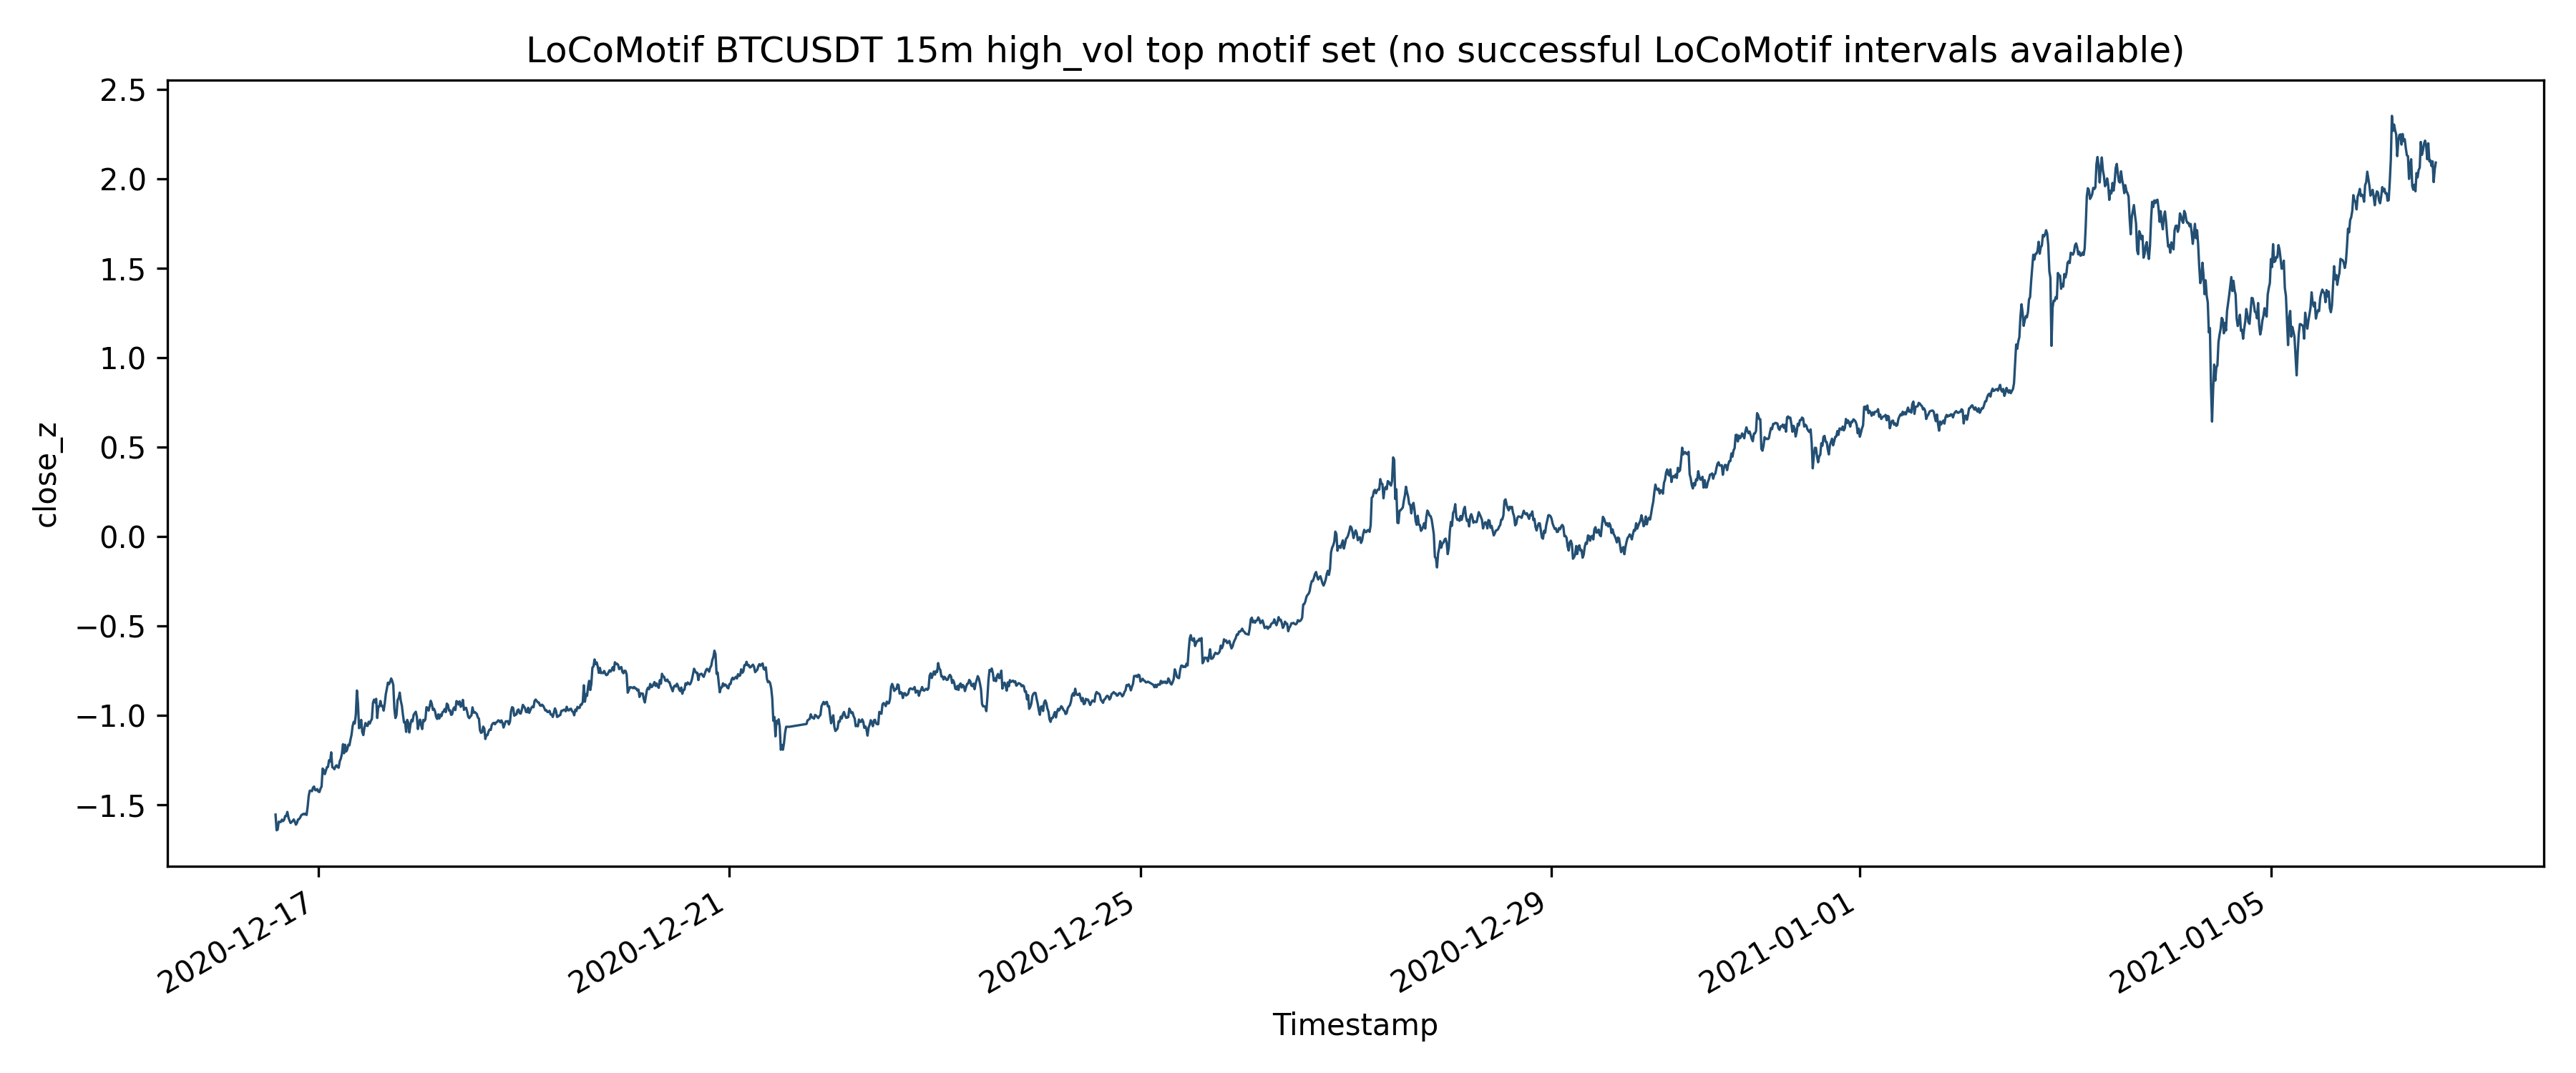
\includegraphics[width=0.95\textwidth]{figures/locomotif_btcusdt_15m_high_vol_top_motif_set.png}\caption{Controlled high-volatility LoCoMotif motif-set overlay.}\end{figure}

\begin{figure}[htbp]\centering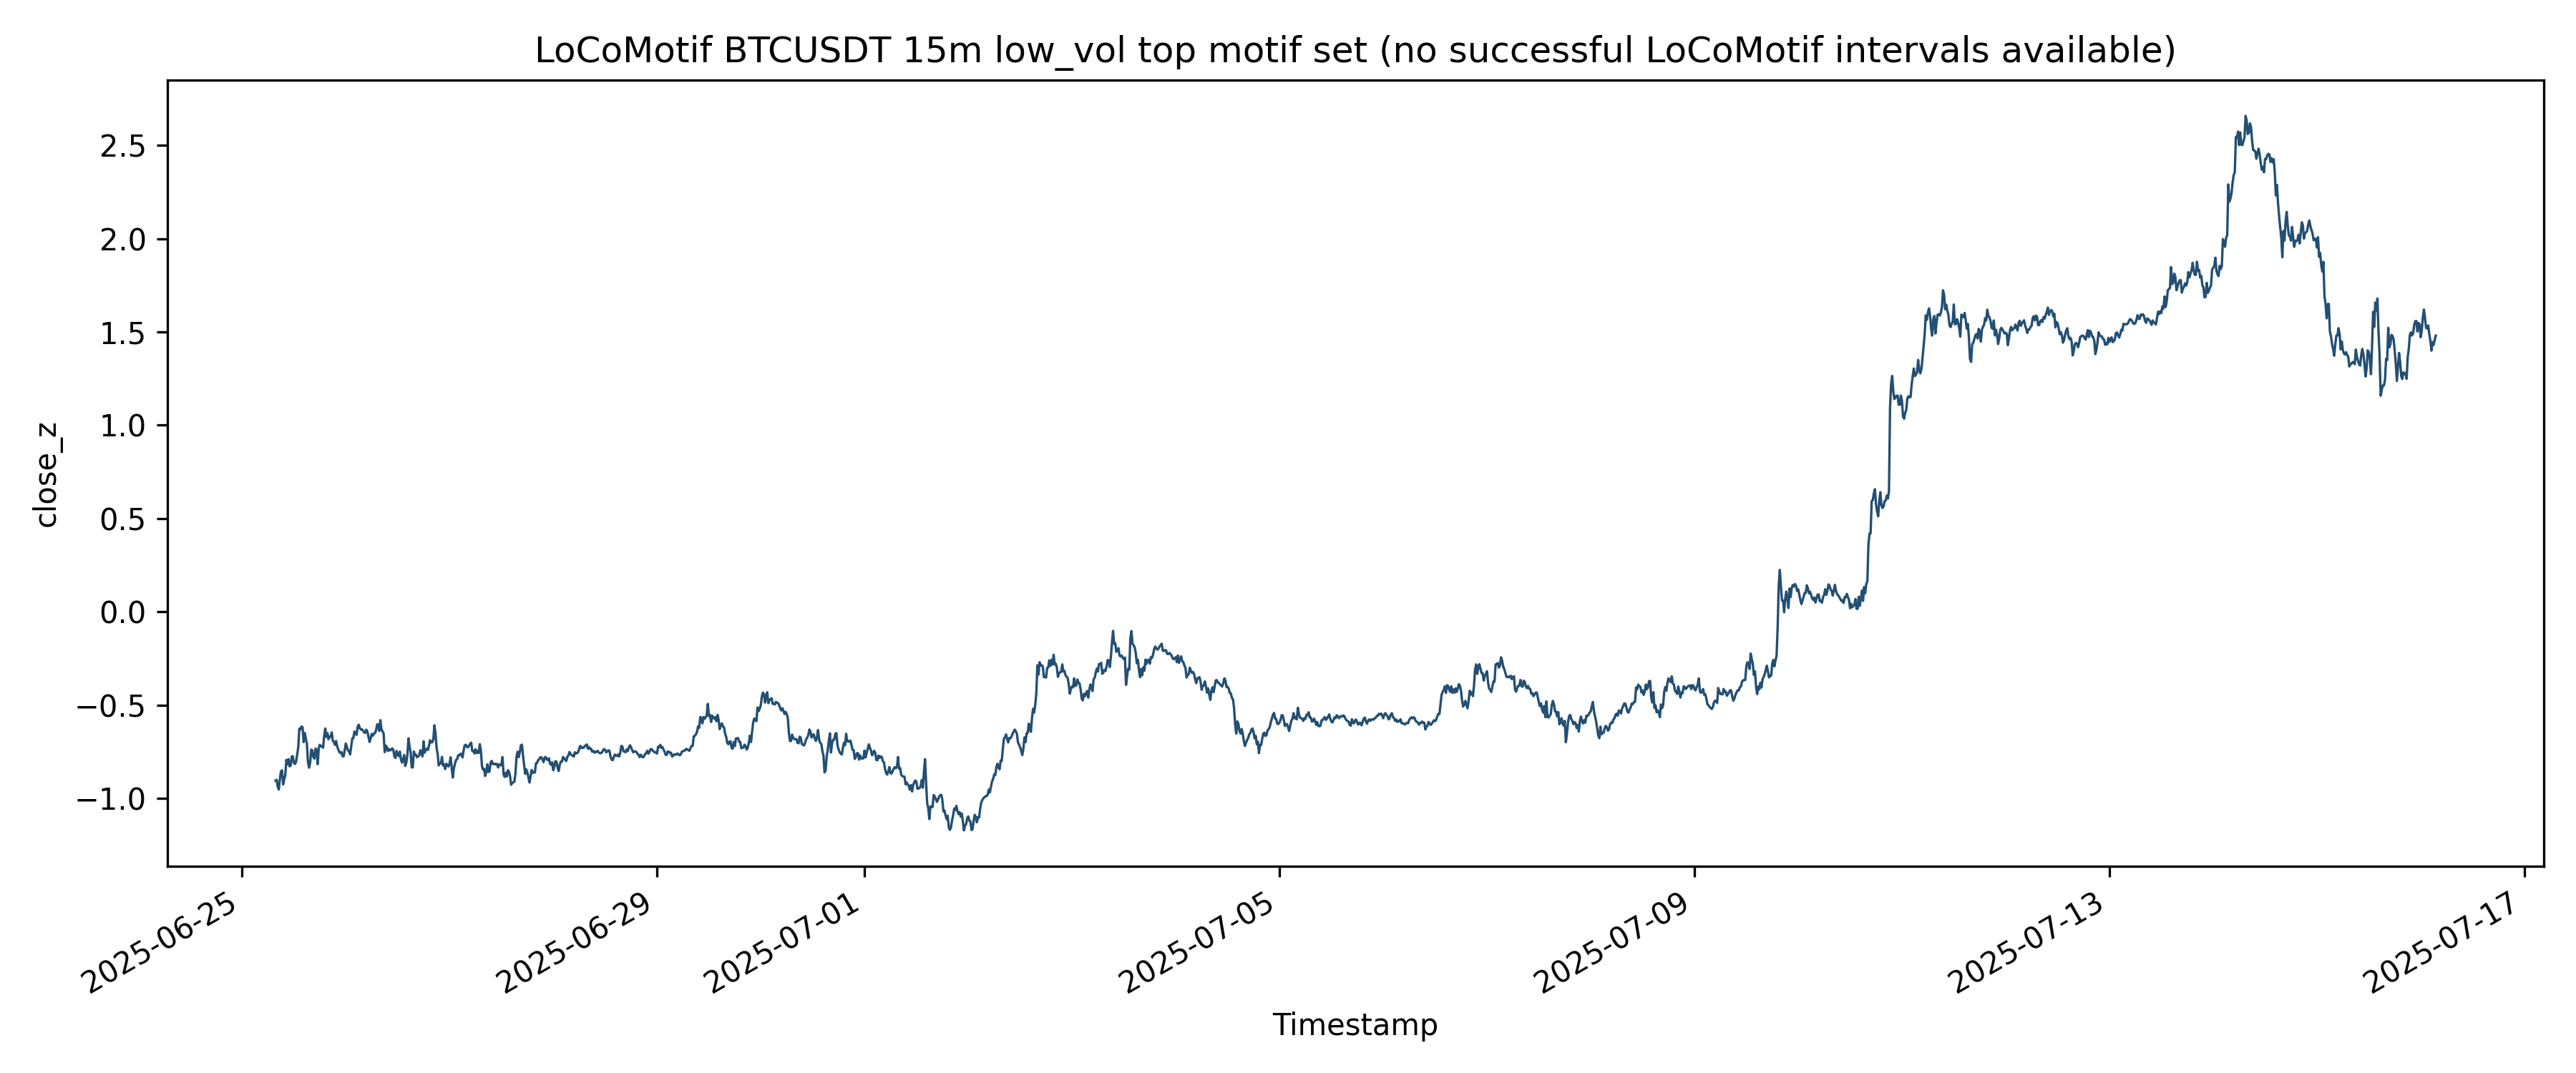
\includegraphics[width=0.95\textwidth]{figures/locomotif_btcusdt_15m_low_vol_top_motif_set.png}\caption{Controlled low-volatility LoCoMotif motif-set overlay.}\end{figure}

\begin{figure}[htbp]\centering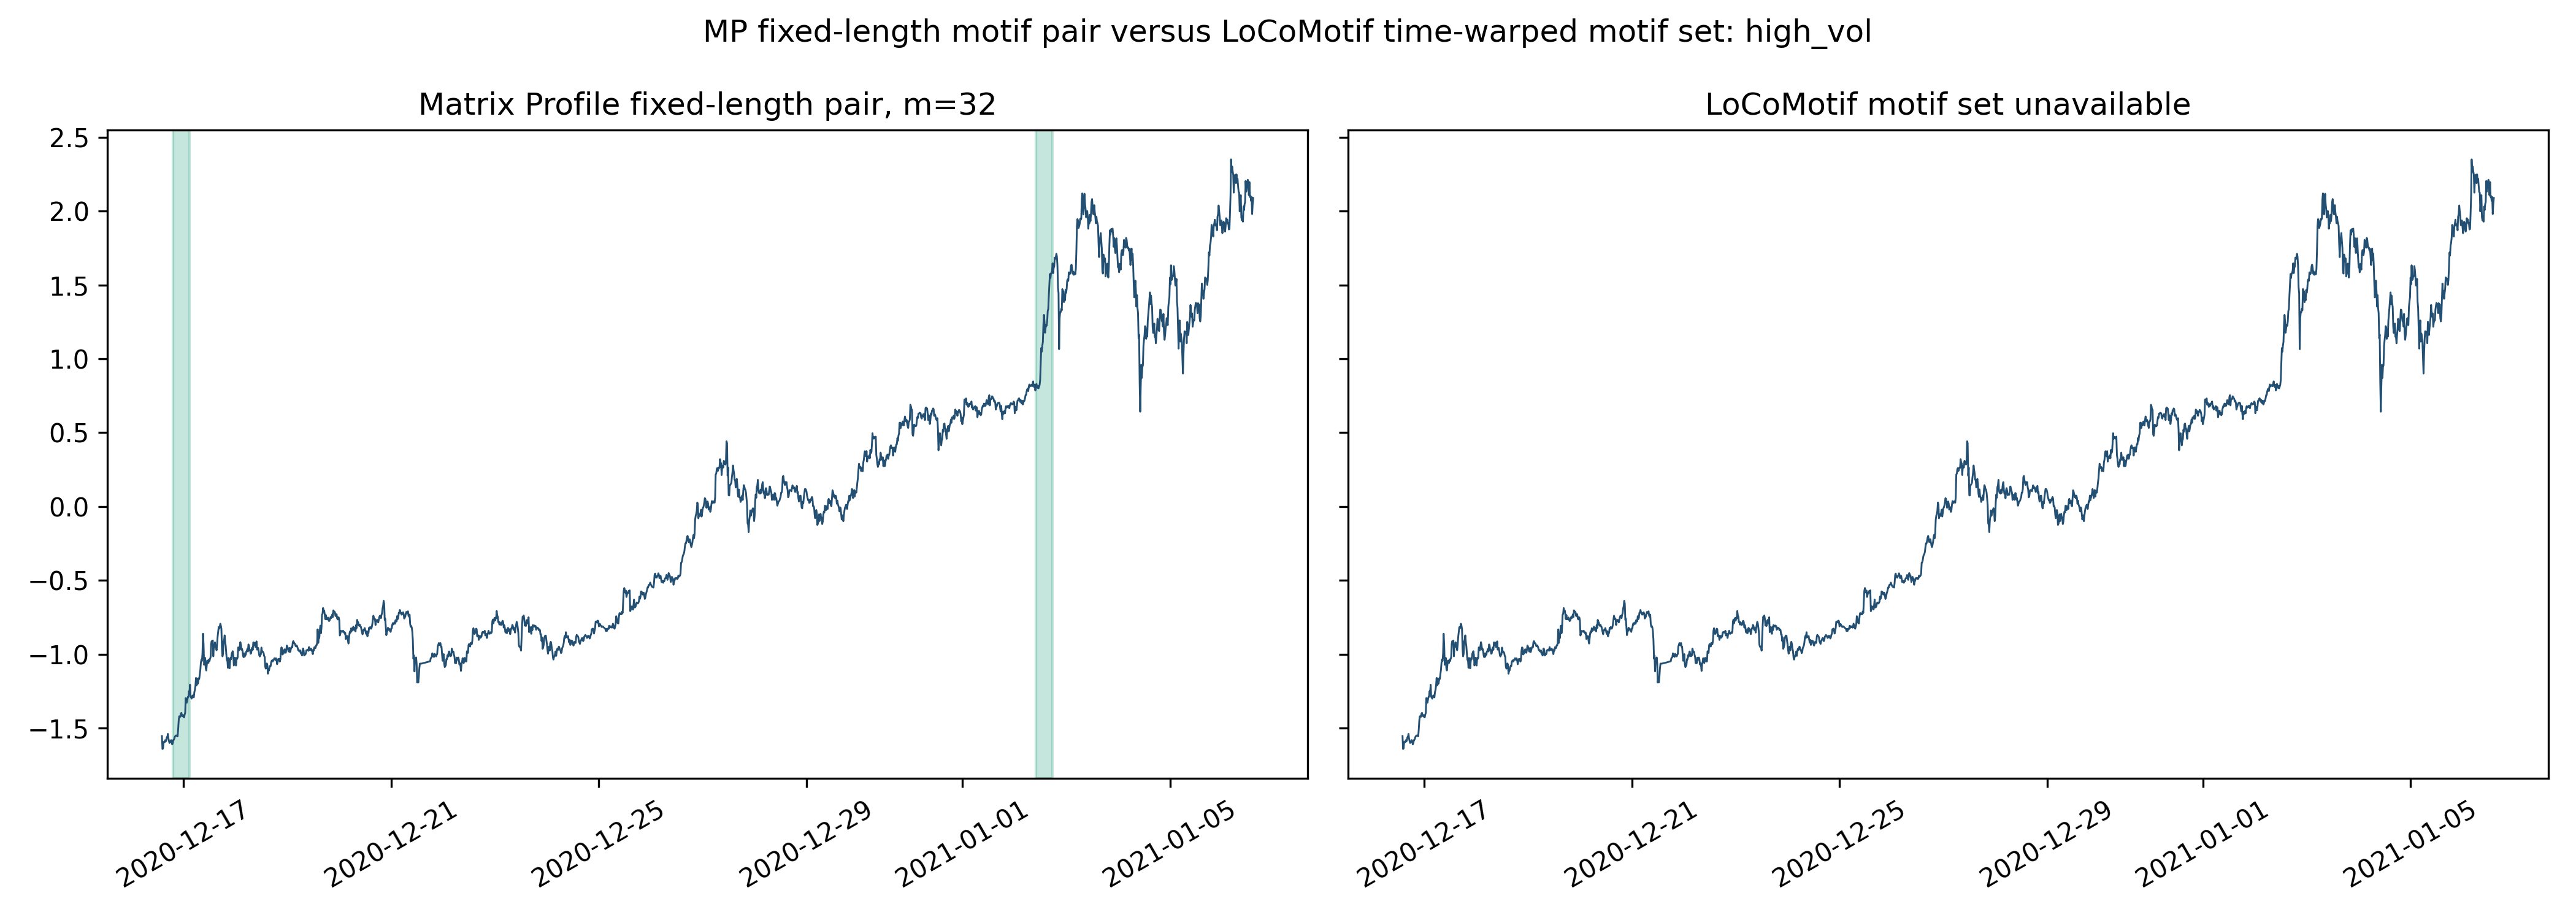
\includegraphics[width=0.95\textwidth]{figures/mp_vs_locomotif_high_vol_side_by_side.png}\caption{Matrix Profile versus LoCoMotif on the high-volatility slice.}\end{figure}

\begin{figure}[htbp]\centering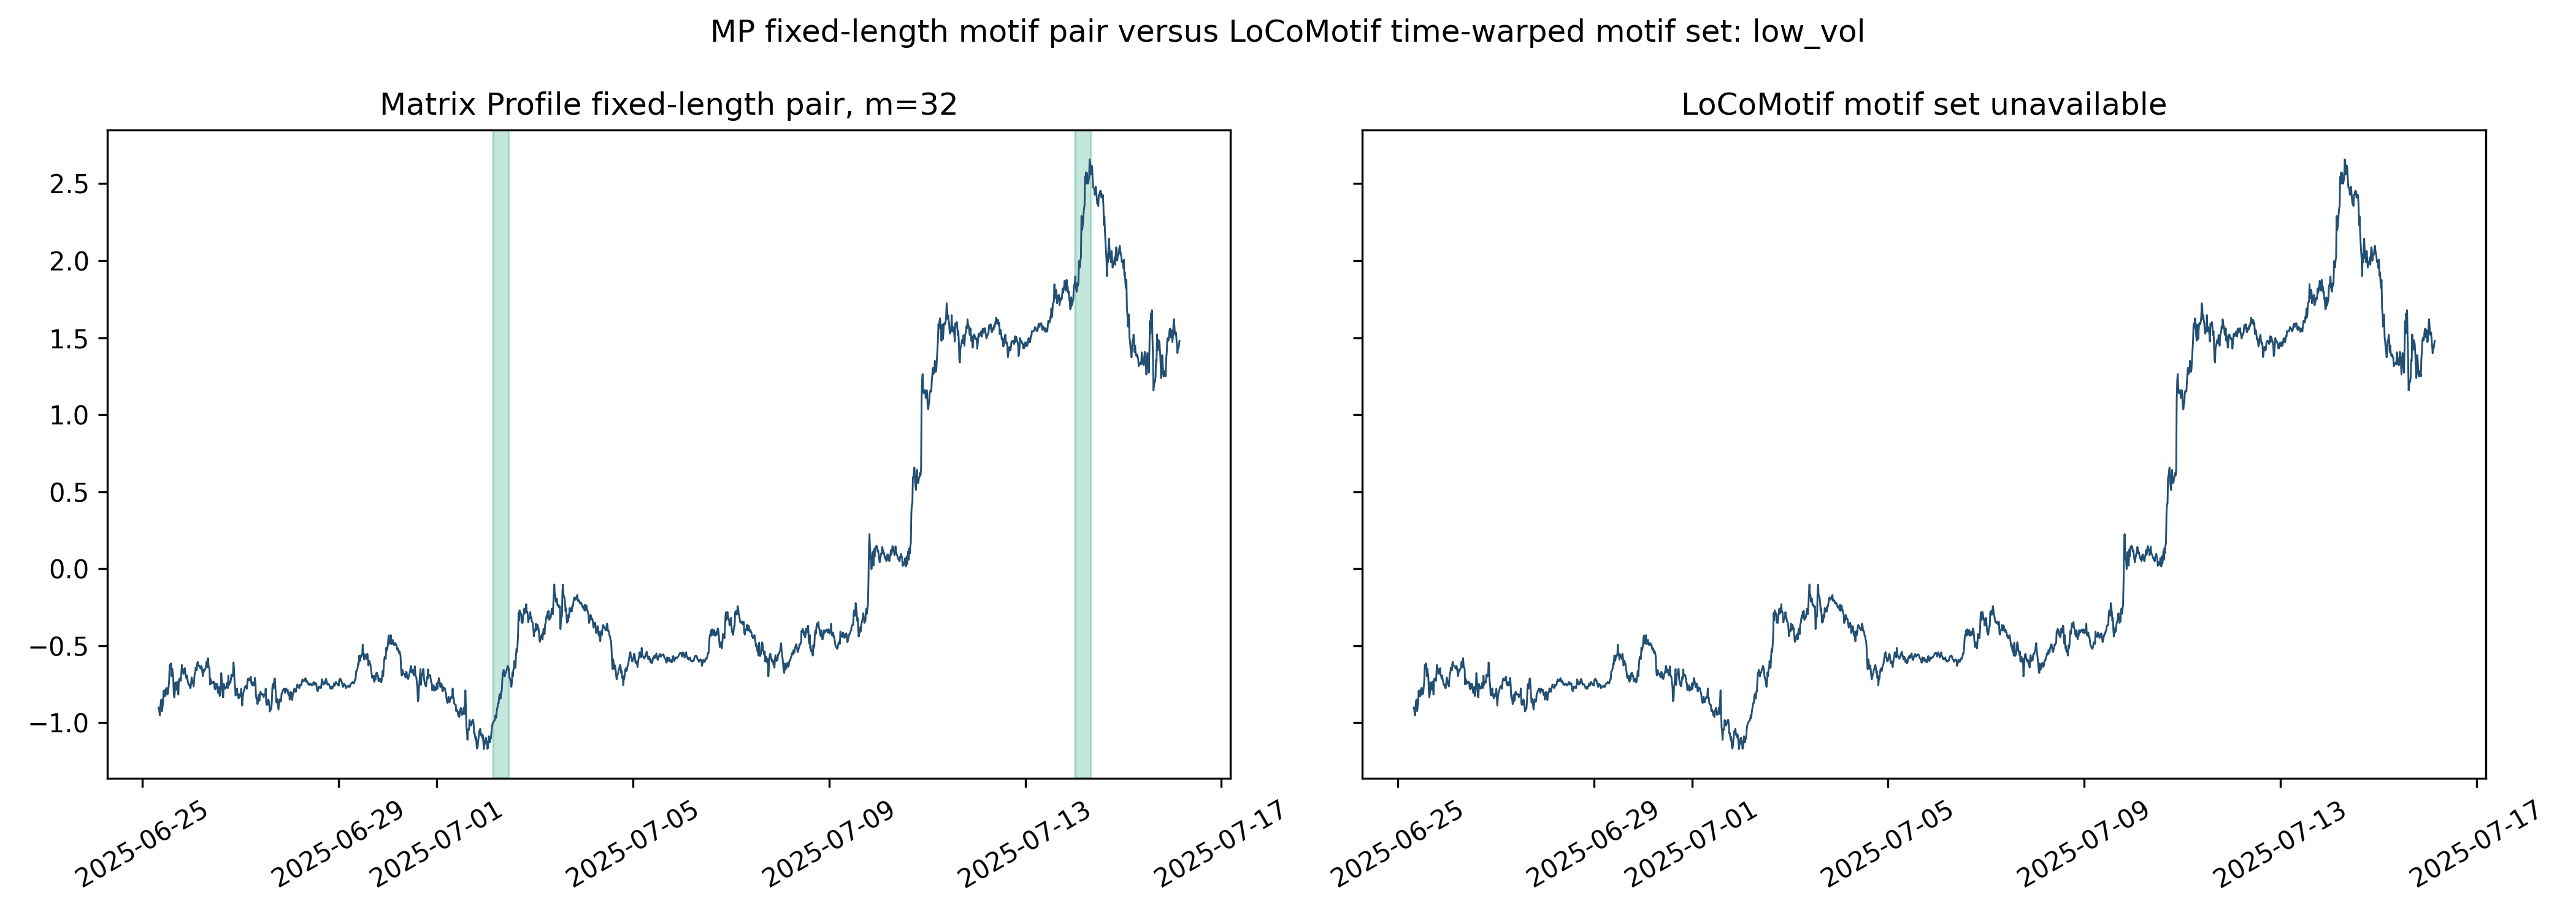
\includegraphics[width=0.95\textwidth]{figures/mp_vs_locomotif_low_vol_side_by_side.png}\caption{Matrix Profile versus LoCoMotif on the low-volatility slice.}\end{figure}